\chapter{Proposed architecture solution} \label{architecture}

For gaining data points for the research, a test setup must be
configured. This chapter presents a Nix ecosystem, which goes through
a red team testing in chapter \ref{analysis}. The proposed
architecture solution uses a completely declarative approach
introduced in section, where pros and cons of both approaches are
discussed \ref{declarativesystems}.

The proposed architecture is a referential framework for a Nix
ecosystem and provide only a basis for a subset of features needed in
such system. For example, remote access and tunneling would require
extra work in a production setting. Note that presented solution's
scalability could be improved with the use of tools referred in
section \ref{nondeclarative}.

The main purpose of the architecture is to construct a system that
focuses on reliability and fluid deployment tasks. Kandoi and Hartke
discuss the operating large scale IoT solutions through declarative
configuration APIs and conclude that it can solve multitude of
scalability and extensibility challenges of IoT systems thus ensure
reliable and safe operations \cite{kandoi2021operating}. As embedded
security is the focal point of this thesis, a further analysis is
presented in chapter \ref{analysis}.

\section{Server}

Van der Burg et al. provide a reference architecture with OpenSSH,
Quake 3 server and Transmission services
\cite{van2013reference}. Dolstra, Vermaas and Levy build a declarative
system with simple web server \cite{dolstra2013charon}. This thesis'
architecture is moderately complex in comparison with these
approaches, as it contains multiple components and a functioning
server–client implementation.

A proposed architecture can be viewed in figure
\ref{parchitecture}. In simplicity, the NixOS server runs a
MQTT-broker for publishing images encoded in base64 format for the
client devices. The clients are called as device fleet, and the server
is called central server. The client devices submit to configured
topics, and display them using a Wayland compositor, Weston.

The central server has two main functions: receiving SSH-connections
for admin usage and forwarding bitmaps formatted in base64 to the
clients. In production environment, the server would be the element
that is in a public network, and the devices would be accessible
locally (through a tunnel). SSH-connections to the machine would then
be forwarded through the central server to the clients. The central
server currently doesn't generate the imagery, but this could be
achieved via headless browser, or other graphical tools.

MQTT is a extremely lightweight, machine-to-machine publish/subscribe
protocol which can be used on virtually every platform including
microcontrollers \cite{oasisopenMQTTVersion}. The chosen MQTT broker
and client for this project is Mosquitto. The following snippet shows
how the Mosquitto server is configured in the NixOS server.

\begin{lstlisting}
  services.mosquitto = {
    enable = true;
    listeners = [
      {
        users.<user> = { acl = [ "readwrite #" ]; }; settings = {
          cafile = "<ssl-path>/ca.crt";
          certfile = "<ssl-path>/myhostname.crt";
          keyfile = "<ssl-path>/myhostname.key";
        };
      }
    ];
  };
\end{lstlisting}

The ''services'' statement tells us that a SystemD service is being
defined. The settings section specify which certificate and key files
are to be loaded to the service.

The MQTT-broker (Mosquitto in this case) publishes a message that is
forwarded to the subscribing clients via a following script.

\begin{lstlisting}
nix shell nixpkgs#mosquitto --command mosquitto_pub -h localhost -t
images/test -m "$IMG_BASE64"
\end{lstlisting}

Sending could be automatized with a service using SystemD timer:
\begin{lstlisting}
systemd.timers.publish-image = {
  timerConfig = {
    OnCalendar = "*-*-* *:*:00";
  };
  wantedBy = [ "timers.target" ];
};
\end{lstlisting}

which invokes a specified service.

\section{Client}

Some IoT solutions prefer client's such relationship with client and
server, where the client automatically searches for suitable server
dynamically \cite{kandoi2021operating}. This thesis' client structure
is static meaning it follows static addresses and forming initial
connections requires manual intervention.

Both server and client are running NixOS. The client has two main
functions: subscribing to media receiving and displaying the gained
media which can be arbitrary. Currently, the image refreshes every
second and through configuration, even displaying animations with this
setup could be possible. Media display happens with feh, an image
showing tool, that works with X server. However, this example is using
Wayland, so compability layer XWayland must be used
\cite{waylandWayland}. Image data messaging functions through
MQTT-protocol, which is explained more in the next subsection.

\subsection{MQTT-client}
The MQTT client subscribes to a topic from the following script. The
image is received as base64 string, and is converted back to PNG
format.
\begin{lstlisting}
IP="<server ip>" TOPIC="images/test" nix shell nixpkgs#mosquitto
--command mosquitto_sub -h $IP -t $TOPIC >" <image directory path>
/image.base64" base64 -d "<image directory path>/image.base64"
>images/latest.png
\end{lstlisting}
\subsection{Weston/XWayland}
Wayland is a display protocol aiming to replace partially or fully the
old X window system. Wayland functions thorugh a "compositor"
(server), and that provides a surface for the device to draw
graphics. Wayland was selected for this project due to increased
security, as the X window system has support for network transparency
which broadens the attack surface. Wayland has combined server and
client rendering with the Wayland compositor, so that safety-critical
throughput between display server and window manager is not a
concern. \cite{waylandWayland} %% waylandmanual

The example project displays an image from a directory via script:
\begin{figure}[H]
\begin{lstlisting} 
    sleep 5 && /nix/store/qc9j6pm6ykyx531s4kb06084mczy2l6g-feh-3.10.1 /bin/feh -F -Z -R 1 <image-path>/latest.png
\end{lstlisting}
\label{fehscript}
\end{figure}
As the programs must be found from an absolute path, the system must
generate the scripts accordingly. This is done via a SystemD service,
specified as:

\begin{figure}[H]
\begin{lstlisting} 
{ config, pkgs, ... }: let
  # Create the feh.sh script to launch feh
  fehLaunch = pkgs.writeText "feh.sh" ''
    echo "sleep 5 && ${pkgs.feh}/bin/feh -F -Z -R 1 <image directory>/latest.png" > /home/user/abzug-receiver/weston/img.sh
  '';

  # Create the initImg.sh script to compile the C code
  initImg = pkgs.writeText "initImg.sh" ''
    echo "${pkgs.gcc}/bin/gcc <source path> img.c -o <binary path>/img" > /home/user/abzug-receiver/weston/init.sh
  '';
in {
  systemd.services."westonl" = {
    enable = true;
    unitConfig = {
      Type = "oneshot";
    };
    serviceConfig = {
      # Set environment variables
      Environment = "XDG_RUNTIME_DIR=/var/run/user/1000";

      ExecStartPre = [
        "${pkgs.bash}/bin/bash ${initImg}"
        "${pkgs.bash}/bin/bash <init.sh path>/init.sh"
        "${pkgs.bash}/bin/bash ${fehLaunch}"
        "${pkgs.bash}/bin/bash <init.sh path>/init.sh"
      ];

      ExecStart = "${pkgs.weston}/bin/weston --config=<weston configuration directory>/weston.ini";

      RestartOn = "failure";
    };

    wantedBy = [ "graphical-session.target" ];
  };
}
\end{lstlisting}
\label{systemd1}
\end{figure}

This wouldn't be a problem in traditional Linux distribution, but in
NixOS the program locations vary from machine to machine
\cite{dolstra2010nixos}. A program resides in Nix store, with a
cryptographic hash of all build inputs in its directory
path. \cite{dolstra2010nixos}. For that reason, one way of proceeding
is to write a SystemD service to generate the configuration
files. Note that this SystemD configuration differs in how SystemD
scripts are declared usually. Most SystemD distributions have SystemD
files in /lib/systemd/system directly or via a symbolic link.

In the beginning of the configuration, variables are defined and
program locations are expanded from Nix package paths. Then, in the
''serviceconfig'' part of the configuration, the strings are forwarded
to shell, which in part compiles sources and executes scripts. After
the ''ExecStartPre'' section, in the ''ExecStart'', Weston is launched
with very basic kiosk configuration:

\begin{figure}
\begin{lstlisting} 
  [core] idle-time=0 xwayland=true [shell] panel-location=""
  panel-position=none** [autolaunch] path=<feh launcher path>/img
\end{lstlisting}
\label{westonconf}
\end{figure}

the ''[autolaunch]'' only functions with compiled binaries thus the
shell script is not directly executed. Instead, a program written in C
is invoked, which in part invokes the shell script with
parameters. The autolaunch path can handle switches, but unfortunately
not parameters. With these workarounds the kiosk successfully can
display media as shown in figure \ref{testimage}. Feh is launched with
-R 1 parameter, which causes it to refresh the image every
second. That way when a new image is uploaded, the display is also
refreshed.

\begin{figure}
    \centering 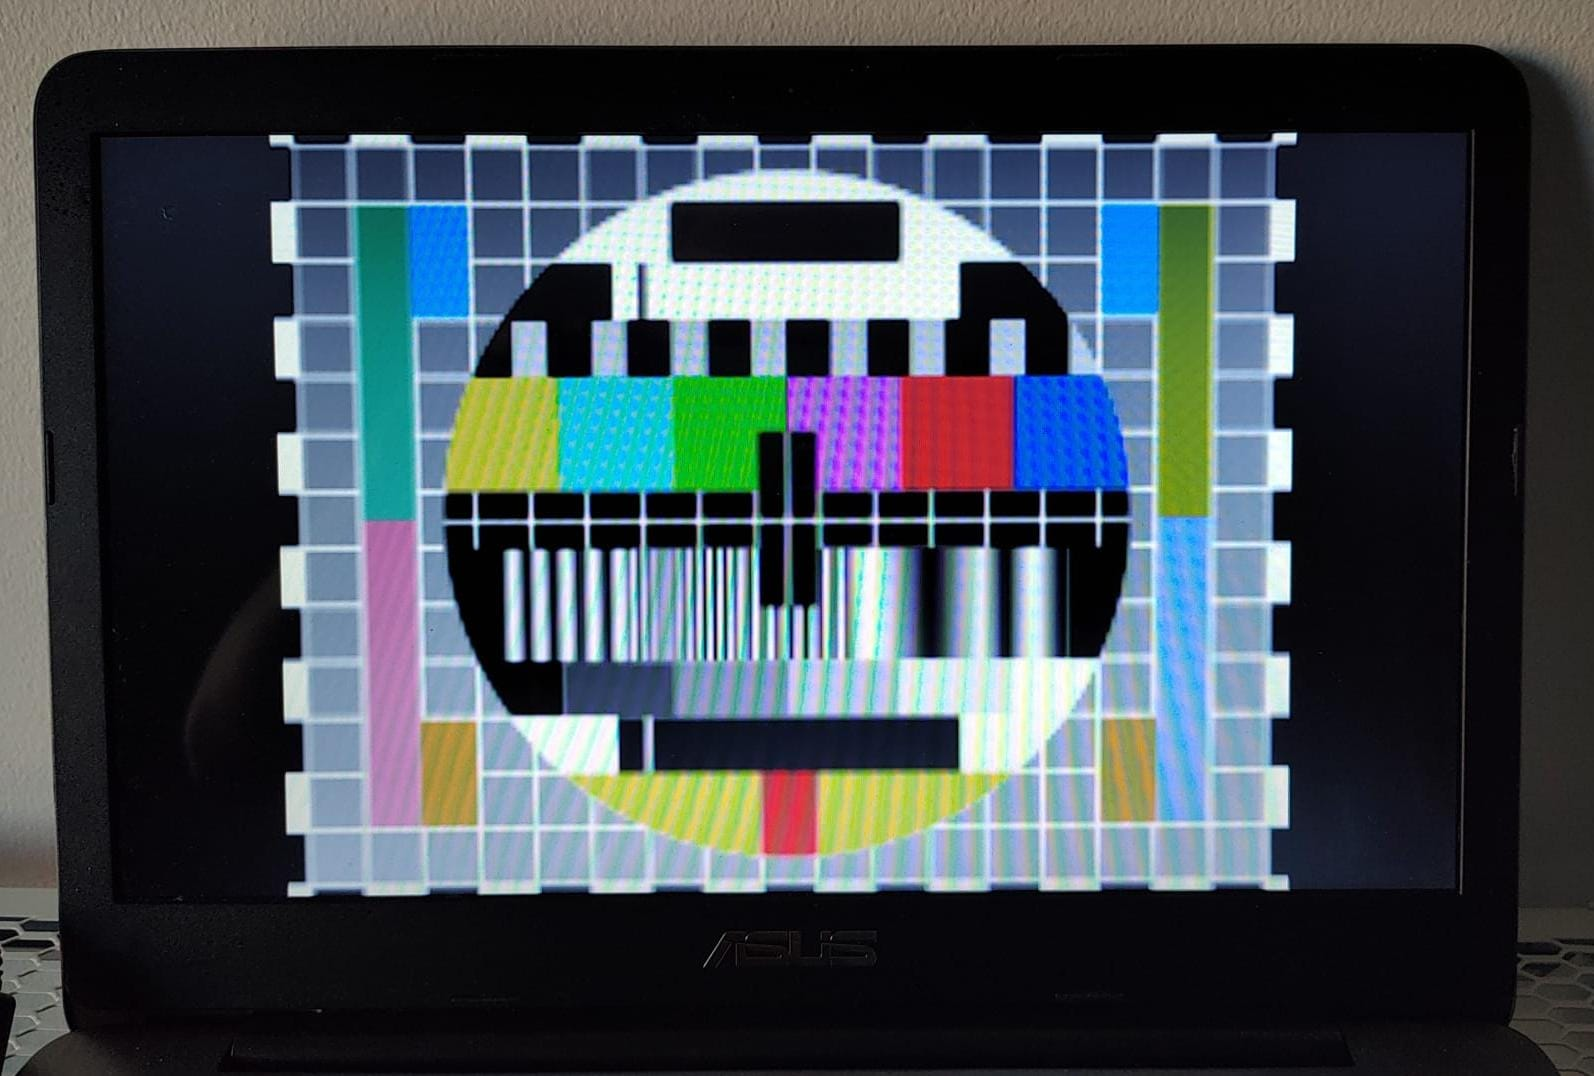
\includegraphics[scale=0.2]{latex/kuvat/testimage.jpeg}
    \caption{Working example of a NixOS client displaying image with
      Wayland and Feh.}
    \label{testimage}
\end{figure}

The sources and scripts are downloaded from Github, again via a
SystemD service. Following snippet shows the "ExecStart" part of the
service.

\begin{lstlisting}
ExecStart="${pkgs.git}/bin/git clone <git url> <installation path>";
\end{lstlisting}

%\begin{figure}[t!]
%\centerline{\includesvg[width=0.70\columnwidth]{latex/kuvat/thesismain.drawio.svg}}
%\caption{Architectural graph of the test setup.}
%\label{parchitecture}
%\end{figure}

\begin{figure}
\includesvg{latex/kuvat/architect.svg}
\caption{Architectural graph of the test setup.}
\label{parchitecture}
\end{figure}
%\begin{figure}
%    \centering
%    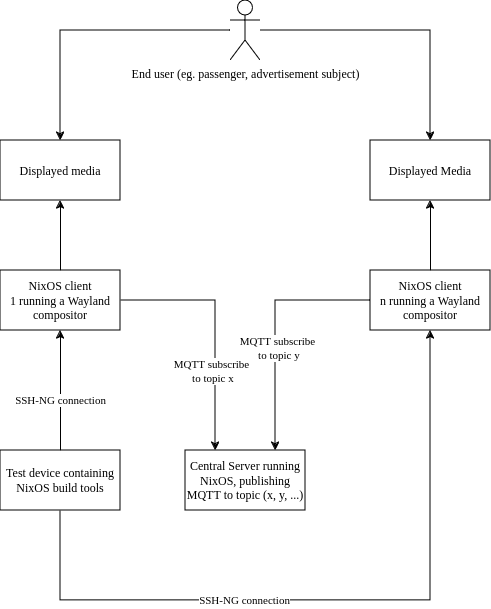
\includegraphics[scale=0.8]{latex/kuvat/architecture.drawio.png}
%    \caption{Architectural graph of the test setup.}
%    \label{parchitecture}
%\end{figure}

This part of the configuration is not purely functional, as the
downloaded scripts and configuration can be arbitrarily changed with
correct permissions. The SystemD services impurity don't trigger the
Nix language evaluation itself, so ''--impure'' switch isn't
mandatory.

\section{Test device}

A huge benefit from declarative systems is their broad possibilities
of automated system tests \cite{van2010automating}. The phrase: "if it
works on one machine, it will work on another" builds a stable
foundation for such tests \cite{nixosNixOSManual}. Different
deployment strategies benefit from slightly different approaches, but
as deployment strategies generally are out of this thesis' scope, only
a minimal test setup is configured.

NixOS devices can be upgraded and updated through a server or locally
with physical access \cite{nixosNixOSManual}. In this thesis' example,
a separate test machine is configured, and it's programs are
replicated to other devices as seen on figure
\ref{parchitecture}. Updates are done manually with command:

\begin{lstlisting}
nix build --eval-store auto --store ssh-ng://remote-host
\end{lstlisting}

The test device is thus replicated to all remote hosts manually, but
an automation script would be useful as the setup scales.

\section{Installing new devices} \label{instnewdevices}

Installing devices could made trivial, as it's trivial to generate new
NixOS images from pre-existing configuration files
\cite{nixosNixOSManual}. The problem is, however, that in many cases a
legacy architexture exists, which needs to be overwritten. This
section focuses on research question 3, providing a solution for
migrating from existing architectures.

If the whole setup needs to be replicated to an existing device fleet,
a great help would be open source project ''NixOS anywhere''. NixOS
anywhere specifies minimal specifications: ''Unless you're using the
option to boot from a NixOS installer image, or providing your own
kexec image, it must be running x86\_64 Linux with kexec
support. Fortunately, most modern x86\_64 Linux systems have kexec
support. By providing your own image you can also perform kexec for
other architectures e.g aarch64''. NixOS anywhere also has a
requirement that the devices should be available at a public network
(not only wireless LAN), which wouldn't probably be a problem in
production environments. NixOS anywhere also works only with NixOS
flakes, so this thesis' configuration would need to be contained in a
flake. \cite{githubGitHubNixcommunitynixosanywhere}
%% cite nixos manual
The installation would contain the following steps:
\begin{enumerate}
  \item Run ''curl -L
    https://github.com/nix-community/nixos-images/releases/download/nixos-unstable/nixos-kexec-installer-noninteractive-x86\_64-linux.tar.gz
    | tar -xzf- -C /root /root/kexec/run'' for booting separate kernel
    for installation.
  \item Generate a minimal configuration file: ''nixos-generate-config
    --no-filesystems --root /mnt''
  \item Add ssh-keys to the configuration
  \item Upload the flake from the server to the device ''nix run
    github:nix-community/nixos-anywhere -- --flake <path to
    configuration>#<configuration name> root@<ip address>''
\end{enumerate}
Another way would be setting up NixOS from the installation media and
setting up manually or creating a installation media with Nixos
generators project
(https://github.com/nix-community/nixos-generators). Nixos generators
is available from Nixpkgs, and can thus be installed to a NixOS
development machine or server. Invoking
\begin{lstlisting}
nixos-generate -f iso -c <configuration.nix path>
\end{lstlisting}
would result in a ISO format image, ready for
installation. \cite{githubGitHubNixcommunitynixosanywhere}

The next chapter provides insight on how to measure security as a
whole, transferring the necessary metric systems for this thesis'
purposes. The architecture presented in this chapter then is gone
through further analysis in chapter \ref{analysis}.
